\section{具体的な進め方}

\subsection{現状の開発状況}

説明の順番の都合上\ref{section:current-status}で説明したので,そちらを参照されたい.

\subsection{事業期間中の開発内容}
\label{section:dev-plan-detail}

\ref{section:dev-goal} で述べた開発目標に対する実装方針を簡単に述べる.

\begin{itemize}
      \item X11の2Dアプリケーションに対応する.\\
            X11のプロトコルをWaylandのプロトコルに変換するXWaylandというソフトウェアがあり,
            これをzmonitorsと同時に起動してあげることで,X11のディスプレイサーバを作成したり
            せずに達成できる.実際にXWaylandを用いてX11のアプリケーションのピクセルマップを,
            自作したWaylandコンポジッタから取得できることを確認している.

      \item XRデスクトップ環境としての機能を充実する.\\
            まずはアプリケーションラウンチャーなどの基本的で簡単な機能から実装する.
            ここはプロジェクトの進捗を鑑みて完成度を高めてゆく.

      \item 2D Windowing Systemとの親和性を高める.\\
            % textlint-disable
            GNOMEやKwinといった既存の2Dデスクトップ環境を拡張する形で実装できれば良いが,
            % textlint-enable
            それはかなり難易度が高いと予想されている.今までの開発から2Dのディスプレイサーバを
            作るほうが慣れているので,GNOMEやKwinの拡張が難しければ,バックアッププランとして,
            ZIGEN用の2D Windowing Systemを開発する.

      \item ゲームエンジンでZIGENの3Dアプリケーションを作成できるようにする.\\
            % textlint-disable
            Unityは開発者は多いがソースコードが公開されておらず,
            % textlint-enable
            拡張できる部分から考えてもUnityを用いてZIGENの3Dアプリケーションを作成するのは
            不可能である可能性が高い.Unreal Engineはソースコードが公開されているが,
            ライセンスを見る限り,開発成果をプラグインとして配布できるが,ソースコードを書き換えて
            再配布は不可能である.プラグインとして配布できるかは検討するが実現可能性は高くない.
            % textlint-disable
            Godot
            \footnote{Godot Engine - Free and open source 2D and 3D game engine: https://godotengine.org/}
            はMIT Licenseの完全にオープンソースのゲームエンジンで,開発者は少ないが,
            % textlint-enable
            3Dゲームエンジンとして注目されており,2021年の12月にはメタ社から助成金も出ている.
            Godotはソースコードを簡単みる限り,3Dオブジェクトをどう描画するかの部分が
            分離されており,その部分を書き換えることでZIGENのアプリケーションが作れる
            ようになる可能性がかなり高く,これをバックアッププランとする.

      \item ZIGENのアプリケーションのストアを展開する.\\
            こちらはプロジェクトの進捗が良かった場合のプラスアルファであり,
            事業期間中には行わない可能性もあり,バッファとする.

      \item より多くのHMDへの対応.\\
            ユーザが圧倒的に多いOculus Quest2への対応をまず行う.
            未踏IT人材発掘・育成事業終了後の進捗として,
            ALVR\footnote{ALVR - PC VR Without the Wires: https://alvr-org.github.io/}
            と組み合わせてワイヤレスでOculus Quest2を用いてZIGENを実行できているが,
            解像度が悪い.有線での通信や通信情報の最適化,レンダリングの一部をOculus Quest2側で
            行うなどの施策を考えている.

      \item 既存のXRアプリケーションと一緒に使えるようにオーバレイとして実装する.\\
            これはOpenVRのOverlay機能を使って表示するようにすれば良いだけなので,
            比較的実装が容易である.ただし現状はOpenVRを用いて開発しているが,
            最新の規格であるOpenXRを用いることも検討している.
\end{itemize}

\subsection{開発体制}

開発者5人で作業を分担する.各々の役割分担は以下の通り定めるが,
開発優先度に合わせて柔軟に対応する.\\
木内:"2D Windowing Systemとの親和性を高める","より多くのHMDへの対応"の部分と全体設計.\\
江口:"X11の2Dアプリケーション対応"とその他Windowing Systemの品質向上.\\
伴:"XRデスクトップ環境としての機能充実"の部分.各種デザイン.\\
劉:"ゲームエンジンでZIGENの3Dアプリケーションを作成できるようにする"の部分.\\
渡辺:"既存のXRアプリケーションと一緒に使えるようにオーバーレイとして実装する"の部分と
全体のバックアップ.

なお渡辺に関しては未踏ジュニア\footnote{未踏ジュニア:https://jr.mitou.org/}に
応募しており未踏ジュニアに採択時には本プロジェクトへの参加を取りやめる予定である.
その場合,渡辺の担当箇所は江口が担当する.

\subsection{開発者スキル}

% textlint-disable
木内:
2021年度の未踏IT人材発掘・育成事業で,本提案の元となった「XR向けWindow System
\footnote{XR向けWindow System: \url{https://www.ipa.go.jp/jinzai/mitou/2021/gaiyou_sd-2.html}}
」の開発をおこなった.
またGoogle Summer of Code 2021においてOSSであるJenkinsコミュニティに貢献し,
Jenkinsのプラグインとして1つのOSSプロジェクトをオーナーとして立ち上げる経験をしたり,
大きなコミュニティでの意思決定の仕方を身近に見たりした.その他ベンチャーでのウェブフロント
のバイト経験やCookpadでバックエンドエンジニアとしてのバイト経験が1年半ほどずつある.
なお,木内に関してはフルタイムで本プロジェクトに従事する予定である.

江口:
2021年度の未踏IT人材発掘・育成事業で,本提案の元となった「XR向けWindow System
\footnotemark[9]
」の開発に従事した.
またZOZOテクノロジーズやCookpadでバックエンドエンジニアとして400万以上のページを収集する
大規模なクローラの開発や生鮮食品ECの新規サービスの開発にそれぞれ1年ほど携わった経験がある.
参加した東京大学のビジネスプランコンテストでは,GPSデータを用いた看板広告のインプレッション
推定のプラットフォームを提案し,2位を受賞した
(\url{https://www.ducr.u-tokyo.ac.jp/activity/venture/education/dojo_2018.html}).
他にも複数社での業務委託開発・複数回のハッカソン出場経験がある.AWS Certificated SAA保持.

伴:
以前からインターフェイスデザインとその未来に強い関心があり,XR領域のプロトタイピング動画を
しばしば制作している(\url{https://twitter.com/i/events/1377153281542123522}).
実装面ではソニーCSLでのインターン(Vue),東京大学のコロナ対策アプリMOCHAの
フロントエンドデザイン\/実装(Flutter)などの経験がある.
3年次には学科でのプロジェクトで制作したMediaPipeのアプリケーション
(\url{https://twitter.com/rtr_dnd/status/1283329784890527746})をもとにした研究で,
IEEE VR 2021にて発表を行った(\url{https://ieeexplore.ieee.org/document/9419110/}).

劉:
AppleやMicrosoftでのインターンを経験し,SiriやBingといった大規模サービスの開発に
携わった.また,Citadel AI(\url{https://www.citadel.co.jp/})にチームで二人目の
エンジニアとして参加し,機械学習モデルのテスト・モニタリングツールのバックエンド\/フロントエンド
の実装,GCP上でのインフラ設計や新機能の提案など多方面に従事した.4月からGoogleで
Chrome OS の開発を行う.また,東京大学のビジネスプランコンテストでは,GPSデータを用いた
看板広告のインプレッション推定のプラットフォームを提案し,2位を受賞した
(\url{https://www.ducr.u-tokyo.ac.jp/activity/venture/education/dojo_2018.html}).

渡辺:
中学生時代に C/C++ を独学で学び,ゲーム開発などを経験する.
学生団体 FascodeNetwork(\url{https://fascode.net/})に所属し,Arch Linux 派生の
国産LinuxディストリビューションであるAlter Linux
\footnote{Alter Linux:https://github.com/FascodeNet/alterlinux/}の開発の一部に参加する.
主にi3wmエディションの開発に携わり,Qt及びC++を用いて簡単にルックアンドフィールを操作できる
設定ツール(\url{https://github.com/FascodeNet/alterlinux-i3-manager})を開発した.
高専入学後はReact及びTypeScriptを用いて,クラス内でテスト対策問題を共有できるサービス
TAGether(\url{https://github.com/watasuke102/TAGether})を開発している.
% textlint-enable

\subsection{開発線表}

図\ref{fig:dev-schedule}に示した.

\begin{figure}[htbp]
      \centering
      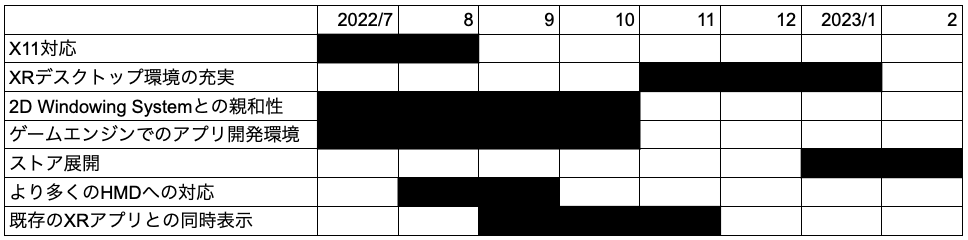
\includegraphics[keepaspectratio, width=\linewidth]{fig/dev-schedule.png}
      \caption{開発線表.黒塗りの時期が取り組む時期.}
      \label{fig:dev-schedule}
\end{figure}

\subsection{克服すべき課題とその解決策}

特に"2D Windowing Systemとの親和性を高める"と
"ゲームエンジンでZIGENの3Dアプリケーションを作成できるようにする"という開発目標は
かなり難易度が高いが,\ref{section:dev-plan-detail}で述べたとおりそれぞれ
バックアッププランを用意している.その他にも基本的に段階的な開発目標立てることで開発が
手詰まりになる可能性を下げている.

% ・計画の緻密さを確認するため、以下の項目を記述してください。
% - 現状のプロトタイプ(あれば)
% - 事業期間中の開発内容
% - 開発体制:目標を達成できる体制になっているか。チームの場合はコミットされた役割
% 分担等も記載してください。他の未踏事業に応募しているメンバーがいる場合、その
% メンバーが抜けた場合の体制についても記載してください。
% - 開発者スキル:プログラミング等開発を行うために必要なスキルをもっているか。また、
% IPA 未踏 IT 人材発掘・育成事業の修了生である場合や、スーパークリエータの認定を受けてい
% る場合はその旨を記述してください。
% - 開発線表 (スケジュール)
% - 克服すべき課題とその解決策
